\section{Introduction}
\label{intro}
The Flatiron building, as seen in \autoref{fig:flatiron}, is the iconic Manhattan skyscraper shaped like a right triangle. Clasped between 5th Avenue and Broadway, with Madison Square Park just north-east of him, there is a lot of open space around this building. If the wind comes from the north, it will be forced through an ``alley'', creating a venturi effect around the Flatiron building. Legend has it that men would hang out out at the corner to watch the wind blowing women's dresses up so that they could see their ankles~\cite{dresses}. This is also shown on a postcard from the early 20\textsuperscript{th} century (\autoref{fig:postalcard}), showing a man being blown away by the wind and a woman's skirt being blown up by the wind.  

The main goal of this research is to see if it was actually the geometry of the building creating the updraft. This will be done by simulating the building and surrounding buildings in an in-house built program made for \emph{Computational Fluid Dynamics} (CFD) analysis for urban areas.

This report will first discuss the theory and numerical models of the CFD simulation, after which it describes the cases and their results, and furthermore these results will be discussed and a conclusion about the billowing of the skirts will be made.

This research is done as part of the Research Laboratory, a course of the Applied Physics study at the Delft University of Technology. The goal is to get students acquainted with the different research groups of the faculty. The results should reflect about 28 hours of work by two students. 

\begin{figure}[h!]
\centering
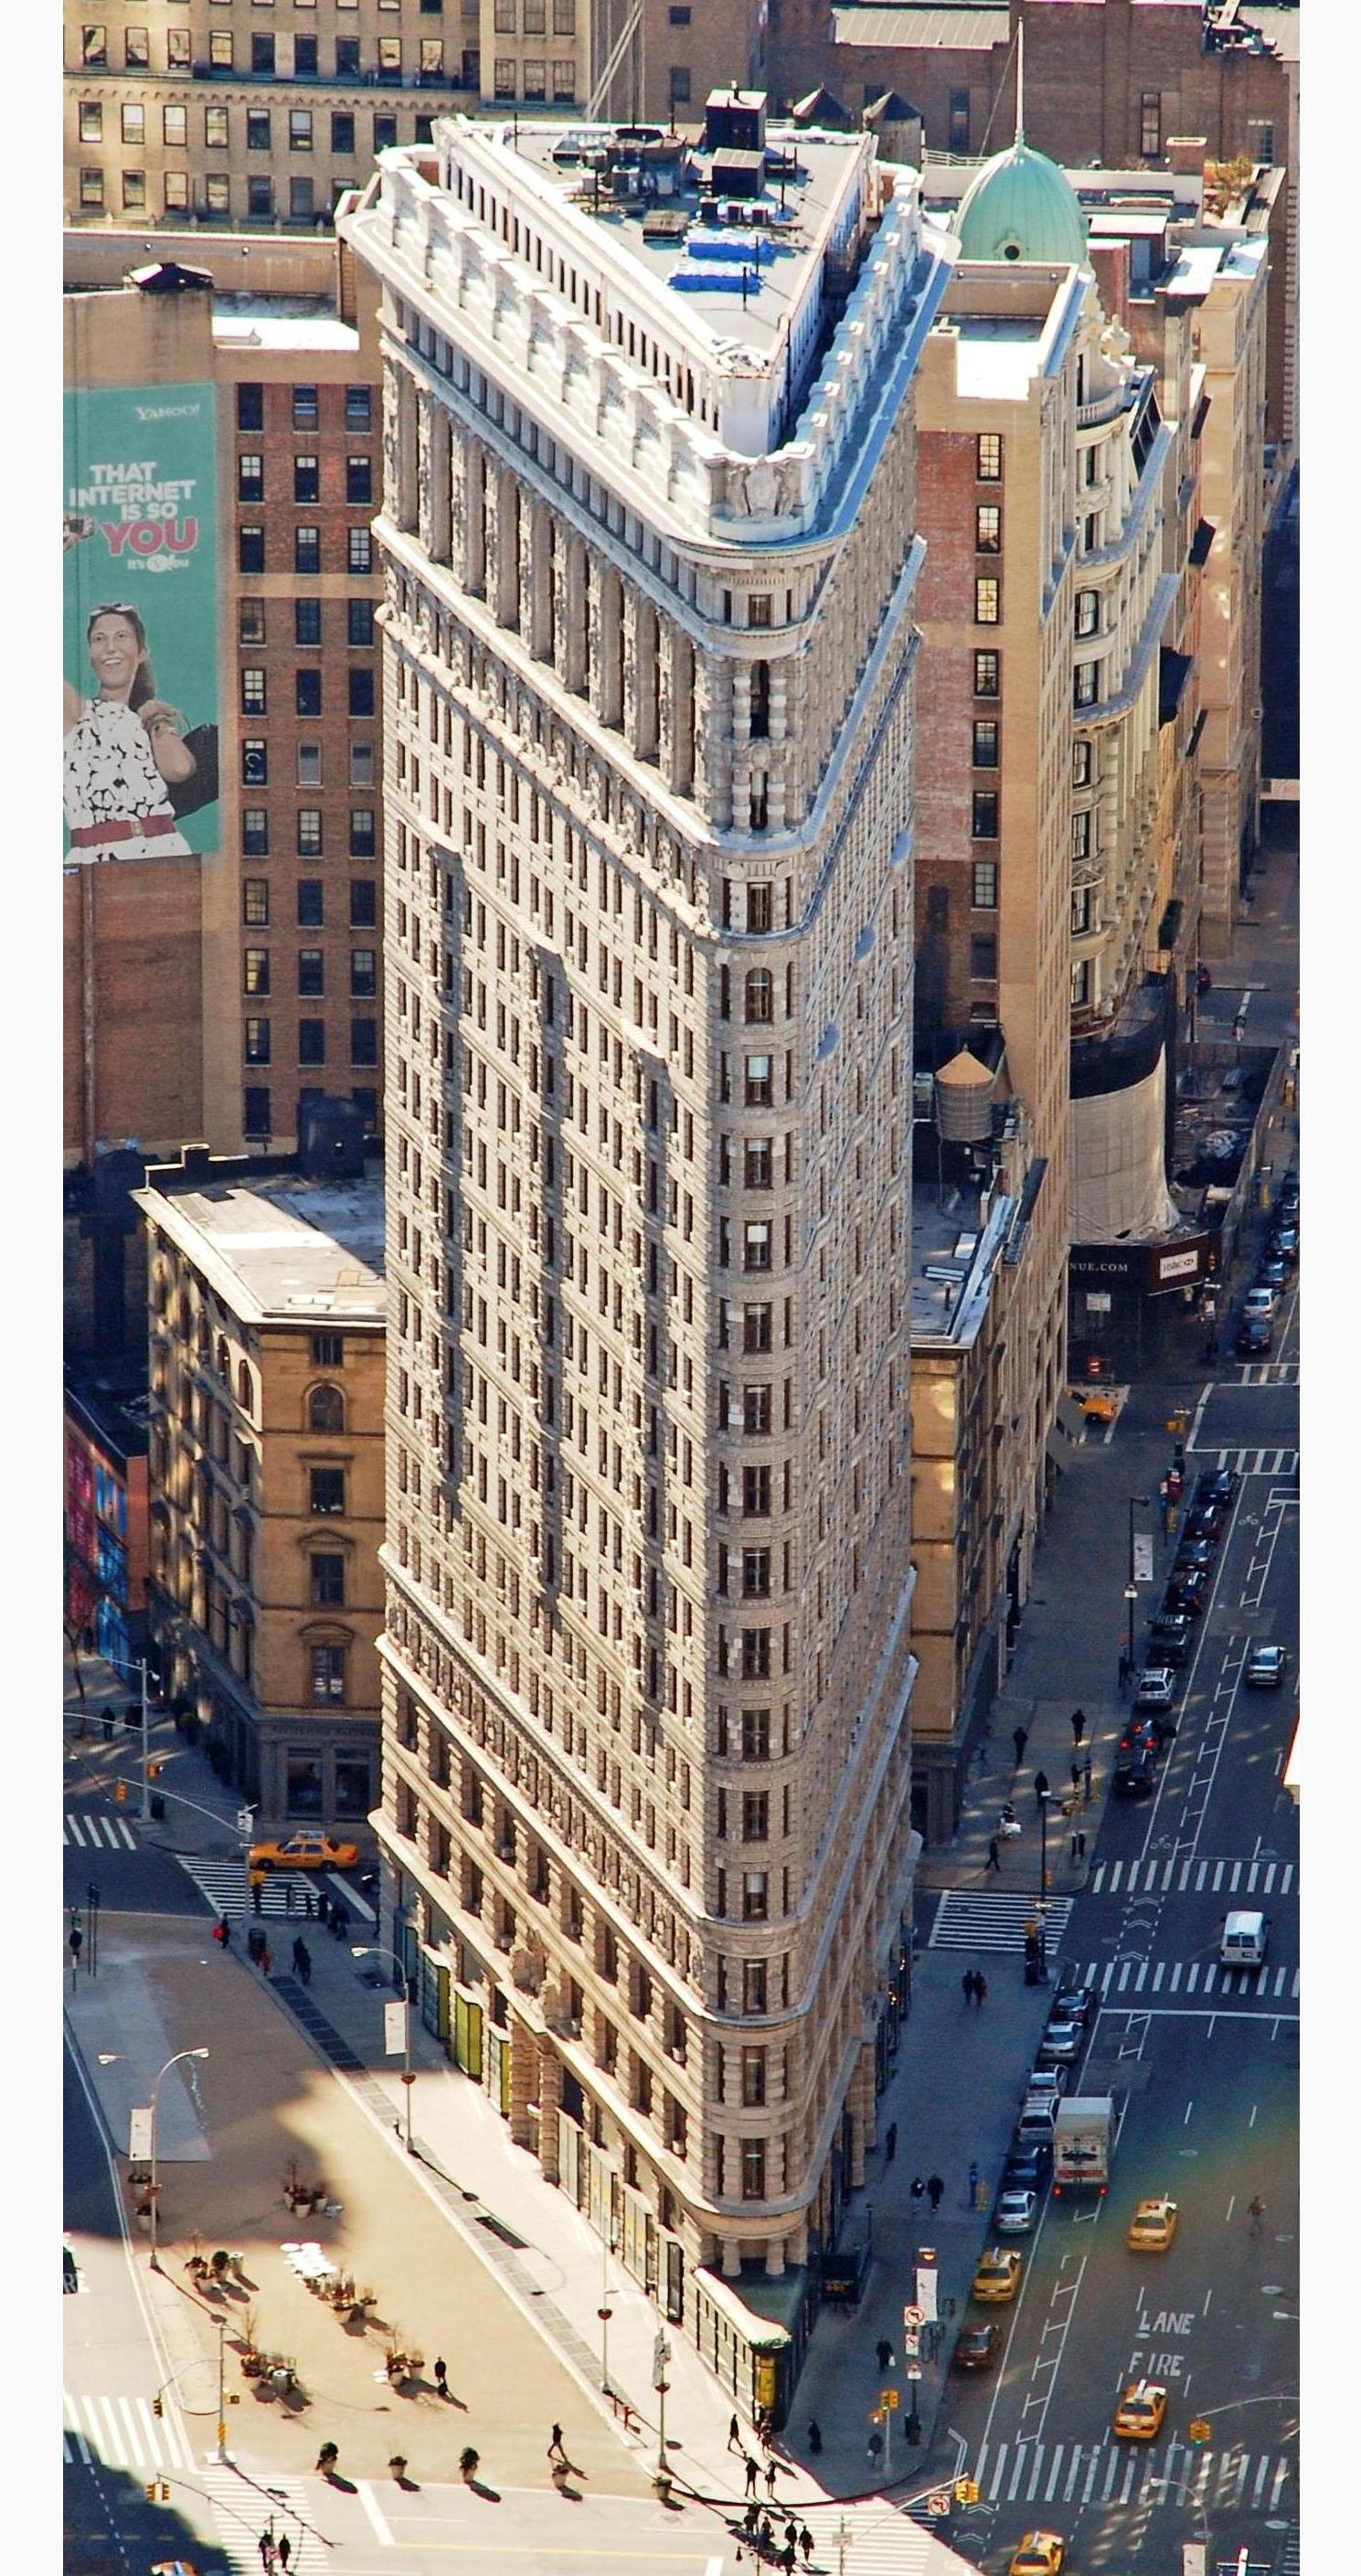
\includegraphics[width = 0.3 \textwidth]{flatiron.jpg}
\caption{A picture of the famous Flatiron building}
\label{fig:flatiron}
\end{figure}
\begin{figure}[h!]
\centering
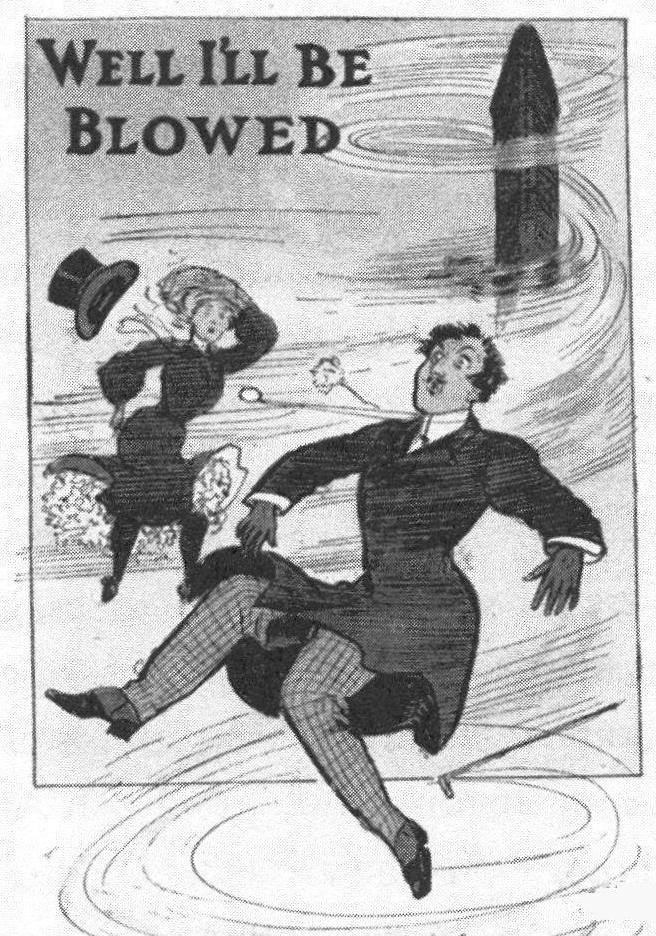
\includegraphics[width = 0.3 \textwidth]{postcard.jpg}
\caption{A postcard by an unknown artist displaying the unpredictable winds and billowing skirts around the Flatiron building \cite{postalcard}.}
\label{fig:postalcard}
\end{figure}